We now propose a parallel algorithm that constructs the {\tt RMMT} of a given tree. Our algorithm, called the
\emph{Parallel Succinct Tree Algorithm} ({\tt PSTA}), has as input a
tree on $n$ nodes stored in the form of a sequence of balanced parentheses, $P$, of
size $2n$.
In practice, it is common to store, in secondary storage, an ordinal tree in the form of a sequence of balanced parenthesis; this scheme is often called the ``folklore'' encoding.
Hence we make such an assumption on the input. 
For trees whose folklore encoding is not directly available, we describe, in Appendix~\ref{subsec:parenthesesAlgorithm}, an algorithm that can compute such an encoding in parallel. 
Our algorithm requires a model that supports
parallelism and can manipulate $w$ bits in $O(1)$ time, where $w$ is the number of bits in a word. DYM meets these
criteria. Additionally, we consider  the overhead (in space and 
time) imposed by the scheduling of cores to be negligible. This is
guaranteed by the results of \cite{Blumofe:1999:SMC:324133.324234}, and in fact the number of available processing units in current systems is generally much smaller than the input size $n$, so this cost is also negligible in practice.

Before describing the {\tt PSTA} algorithm, we observe that, the entries in $e'$ that correspond to the internal nodes of the {\tt RMMT} need not be stored explicitly.
This is because the entry of $e'$ corresponding to an internal node is equal to the entry that corresponds to the last leaf descendant of this node; as the {\tt RMMT} is complete, we can easily locate such a leaf in constant time.
Thus, in the description of our algorithm, we treat $e'$ as an array of length $\lceil 2n / s\rceil$, in which each entry corresponds to a leaf.
Our algorithm then consists of three phases. In the first phase, it computes the leaves of the {\tt RMMT}, i.e., the array $e'$, as well as the entries of $m^{\prime}$, $M^{\prime}$ and $n^{\prime}$ that correspond to the leaves of the {\tt RMMT}.
In the second phase, the algorithm computes the internal nodes of the
{\tt RMMT}, i.e., the remaining entries of $m^{\prime}$, $M^{\prime}$ and $n^{\prime}$. 
Finally, in the last phase, it computes the universal tables used in the {\tt RMMT} in parallel.
In our discussions, we assume that the input of our algorithm includes $P$, a parentheses
sequence of size $2n$; $s$, the size of each chunk; and $threads$, the total numbers of available
threads.
The pseudocode of the sequential version of our algorithms can be obtained by replacing {\bf parfor} instructions by 
sequential {\bf for} instructions in the pseudocode shown in Figure~\ref{fig:psta}.

Algorithm \ref{algo:PSTA1} presents the pseudocode for computing the leaves of the {\tt RMMT}. 
Recall that the size of array $e^{\prime}$ is the number of leaves
in the {\tt RMMT} (line 2), and the size of arrays $m^{\prime}$,
$M^{\prime}$ and $n^{\prime}$ is equal to the total number of nodes in
the {\tt RMMT}, i.e., $2\lceil 2n/s \rceil-1$ (lines 1 and 3).
In this algorithm, we first assign the same number of consecutive chunks to each core.
The number, $ct$, of chunks assigned to each core is computed as $\lceil 2n / s\rceil / threads $ (line 4); we assume that $\lceil 2n / s\rceil$ is divisible by $threads$ for simplicity.
The chunks assigned to each core forms a contiguous subsequence of $P$, and we compute, in parallel, the {\em local} excess value of the last position in each chunk, by letting each core loop through the subsequence assigned to it.
Here the local excess value of a position $i$ is defined to be $\sumop(P,\pi,j,i)$, where $j$ is the index in $P$ that corresponds to the starting position of the subsequence assigned to the core that computes the local excess value at position $i$. 
These local excess values are stored in $e'$. 
During this process, we also compute the minimum and maximum values of the local excess values in each chunk, and store them in the corresponding entries of $m$ and $M'$, respectively.
Note that during this process, we can correctly compute the entries of $n'$ that correspond to leaves. 
Lines 4 to 21 show the computation. %, in which each thread computes the excess value of $ct$ consecutive chunks by walking through them, following the above equation to compute local excess values.
%Each time an opening parenthesis appears in a chunk,  the
%thread increments the current local excess value that it is maintaining, and decrements the value otherwise (lines 11 to 14).
%Immediately after the local excess changes, it is
%necessary to verify if the maximum, minimum and number of minimum
%values also change (lines 15 to 21). When a chunk is completed, the
%local excess and its associated values are stored in the arrays
%$e^{\prime}$, $m^{\prime}$, $M^{\prime}$ and $n^{\prime}$ (lines 22 to
%25).
After these steps, the arrays $e'$, $m'$ and $M'$ store the local excess values for the leaf nodes of the {\tt RMMT}, and we next update them to store the corresponding global excess values in $P$. 
To achieve this goal, we first update the excess value of the last position of the subsequence assigned to each core.
We observe that for the $i$th core, the global excess value of the last position in its subsequence  is equal to the sum of the local excess values of the last positions in the subsequences assigned to the first $i$ cores. 
Therefore, we can use a parallel prefix sum algorithm~\cite{Helman2001265} to update all these values (line 22). 
%Note that the prefix sum algorithm computes the prefix sums over only $p$ values. 
After this, each process can then update the remaining excess, minimum and maximum values in
parallel, by making use of the excess value of the last position of the subsequence assigned to the previous core (lines 23 to 28).

Algorithm \ref{algo:PSTA2} shows the computation of the internal nodes.
In this algorithm, we first compute the closest
level, $lvl$, to the root that has at least $p$ nodes (line 1).
Note that we number the levels incrementally starting from the root, which is at level $0$.
Then for each node at level $lvl$, we assign the subtree rooted at it to a core.
This core computes the entries of $m$, $M'$ and $n'$ that correspond to each node in this subtree, by processing the entries of $m$, $M'$ and $n'$ corresponding to its two children.
Lines 2 to 6 show the details, in which line 6 calls the function $concat$, whose pseudocode is also given.
Notice that one core can possibly compute
more than one subtree and those subtrees may be non-consecutive. With
a scheduler that balances the work, such as a work-stealing scheduler, cores have a similar workload.
Finally, for each of the remaining levels (levels $lvl-1, lvl-2, \ldots 0$), the algorithm computes the entries of $m$, $M'$ and $n'$ that correspond to the nodes at each level in parallel (lines 7-10). 

In the last phase of {\tt PSTA}, Algorithm \ref{algo:PSTA3} shows the computation of
universal tables.
As each entry in a universal table can be computed independently, we can easily compute them in parallel. 
To simplify the explanation, Algorithm
\ref{algo:PSTA3} just shows the computation of one universal table,
$near\_fwd\_pos$, which is the one used to support the {\fwdsearch} operation (its content is described in Section~\ref{subsec:suctrees}). The same algorithm can be applied to the other
tables.
%
%All of these tables do not depend on the input, except for the
%number of available threads.
%
%
%The {\tt RMMT} is constructed over $P$, partitioning $P$ in disjoint
%chunks of size $s$. Considering those chunks, the construction of the
%{\tt RMMT} is based in the computation of different arrays of size
%$O(\frac{N}{s})$. Such arrays are $e^{\prime}$, saving the final
%excess of each chunk, $m^{\prime}$, saving the minimum excess value of
%each chunk, $M^{\prime}$, saving the maximum excess value of each
%chunk and $n^{\prime}$, saving the number of ocurrences of the minimum
%value of each chunk. As a reminder, the excess value at position $i$
%is:
%\begin{equation}
%  \displaystyle E[i] = \sum_{k=0}^{i} \pi(P[k])
%  \label{eq:excess}
%\end{equation}
%
%where $\pi(``(") = 1$ and $\pi(``)") = -1$. See Figure
%\ref{fig:RangeMinMaxTree} as an example of {\tt RMMT}, with $s=3$ and
%$k=3$.
%
%\begin{figure}[ht]
%  \centering
%  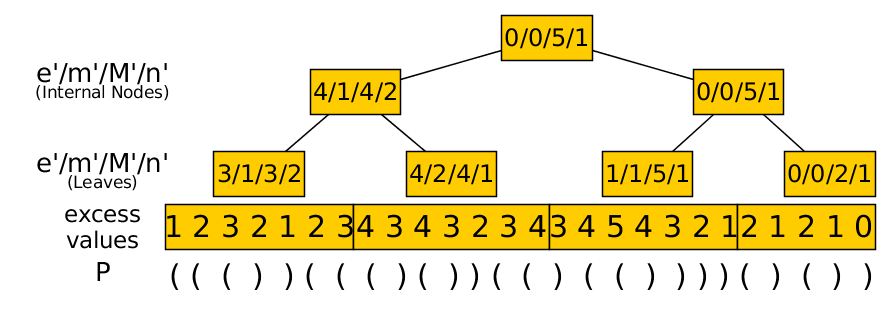
\includegraphics[scale=0.18]{./images/Range-min-max-tree.png}
%  \caption{Range min-max tree}
%  \label{fig:RangeMinMaxTree} 
%\end{figure}
%
%The first step of {\tt PSTA} is to compute the arrays $e^{\prime}$,
%$m^{\prime}$, $M^{\prime}$ and $n^{\prime}$ in parallel. Since
%$e^{\prime}$ just saves the last excess value of each chunk, which is
%a sum, {\tt PSTA} needs to apply a parallel prefix sum
%algorithm. Computing the last element of $e^{\prime}$, at position
%$\frac{2n}{s}-1$, we indirectly compute the rest of the elements of
%$e^{\prime}$. We adapted the algorithm in \cite{Helman2001265} for
%this context, computing $e^{\prime}$ in $O(\frac{n}{p}+\lg p)$ time, using
%$p$ threads. Note that we do not need to compute more elements of
%$e^{\prime}$ to the internal nodes of the {\tt RMMT}. The memory used
%in construction time are bounded by $O(n\lg(n))$ bits.
%
%To compute $m^{\prime}$, let's assume, without loss of generality,
%that $p = k^{i}$, where $k$ is the arity
%of the internal nodes in the {\tt RMMT} and $i > 0$. {\tt PSTA}
%assigns one thread per sub-tree of size $O(\frac{n}{sp})$, at level
%$i$. So, it is possible to compute the $m^{\prime}$ values in all
%sub-trees, in parallel, in $O(\frac{n}{sp}k)$ time. Then, for the
%rest $O(p)$ nodes in the top of the tree, we compute the corresponding
%minimum values in $O(k\lg_{k} p)$ time, computing each level in $O(k)$
%time, just looking the $k$ values on the previous level using one
%thread per vertex. If we consider $s$ and $k$ as constants, we can compute
%$m^{\prime}$ in
%$O(\frac{n}{sp}k + \lg p) = O(\frac{n}{p}+\lg p)$ time,
%using $O(n\lg(n))$ bits in construction time and in the
%final array. Note that this solution makes sense considering that
%$p\ll N$. Figure \ref{fig:min-max-array} illustrates the solution
%explained here. We can compute $M^{\prime}$ and $n^{\prime}$ in the
%same way, obtaining the same complexity.
%
%\begin{figure}[t]
%  \centering
%  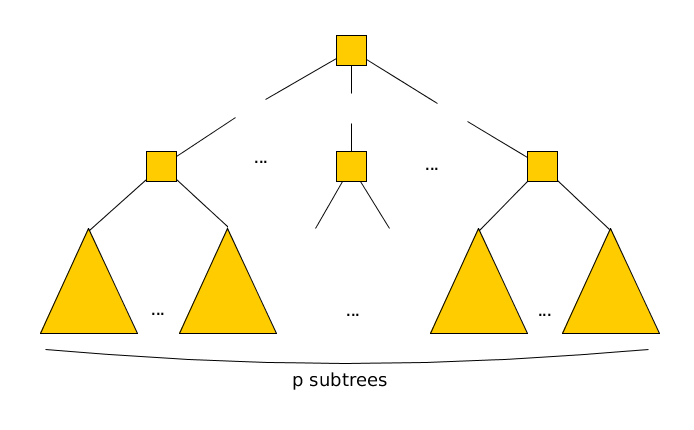
\includegraphics[scale=0.28]{./images/Min-Max-array.png}
%  \caption{Computation of $m^{\prime}$ and $M^{\prime}$}
%  \label{fig:min-max-array} 
%\end{figure}
%
%In addition to the arrays, the construction of the {\tt RMMT} involves
%the computation of \emph{universal tables}.
%The universal tables are
%used to support \emph{fwd\_search}($\bullet$),
%\emph{bwd\_search}($\bullet$), \emph{rmqi}($\bullet$),
%\emph{RMQi}($\bullet$), \emph{degree}($\bullet$) and
%\emph{child}($\bullet$) queries.
%We can divide
%universal tables into two types: those that depend on the leaves of
%the {\tt RMMT} and those that depend on the internal nodes. In the
%first case, we can compute each universal table in parallel assigning
%one processor per leaf or chunk, which allows to compute different
%parts of the table at the same time. For the second kind of tables, we
%can assign one processor per internal node. Such processor computes
%the section corresponding to that internal node in the universal
%table. In that way, since computing the universal tables sequentially
%has a complexity of $O(\sqrt{2^{w}}poly(w))$ time according to
%\cite{Navarro:2014:FFS:2620785.2601073}, we can compute those
%universal tables in $\displaystyle O(\sqrt{2^{w}}poly(w)/p)$,
%using $p$ processors.
%
%To reduce the space used by the {\tt RMMT}, Sadakane and Nava\-rro used
%the \emph{aB-tree}. As the {\tt RMMT} and aB-tree are both complete trees, we can apply a
%construction as that shown in Figure \ref{fig:min-max-array} to
%construct the aB-tree. With respect to the universal tables needed in
%the aB-tree, they can be computed following the same strategy
%explained previously, but now with size $O(\sqrt{2^{w}})$
%bits.

\begin{figure}
\begin{minipage}[t]{.50\textwidth}
  \vspace{0pt}  
  \begin{algorithm}[H]
\small
\SetVlineSkip{-2cm}
  % keywords
  \SetKwInOut{Input}{Input}
  \SetKwInOut{output}{output}
  \SetKwFor{PFor}{parfor}{do}{end}
  \LinesNumbered
  \SetAlgoNoEnd
  \DontPrintSemicolon
  % I/o
  \Input{$P$, $s$, $threads$}
  \output{$e^{\prime}, m^{\prime}, M^{\prime}, n^{\prime}$ and universal tables ({\tt RMMT})}
  \BlankLine% \SetAlgoNoLine
  % algorithm
  $o$ = $\lceil 2n/s \rceil-1$\tcp*[h]{\# internal nodes}\;
  $e^{\prime}$ = array of size $\lceil 2n/s \rceil$\;
  $m^{\prime}, M^{\prime}, n^{\prime}$ = arrays of size $\lceil 2n/s \rceil + o$\;
  $ct$ = $\lceil 2n/s \rceil/threads$\;%\tcp*[h]{Chunks per thread}\;
  \PFor{$t\leftarrow 0$ \KwTo $threads-1$}{
	  $e^{\prime}_t, m^{\prime}_t, M^{\prime}_t, n^{\prime}_t$ = $0$\;
	  
	  \For{$chk \leftarrow 0$ \KwTo $ct-1$}{
		  $low$ = $t*ct*s+chk*s$\;
		  $up$ = $low+s$\;
	  	
		  \For{$par \leftarrow low$ \KwTo $up-1$}{
			$e^{\prime}_t$ += $2*P[par]-1$\;		    
%		  	\eIf{$P[par]$ is $closed$}{
%		  		$e^{\prime}_t$ -= $1$\;
%		  	}
%		    {
%		  		$e^{\prime}_t$ += $1$\;
%		    }
%		    
		    \uIf{$e^{\prime}_t < m^{\prime}_t$}{
				$m^{\prime}_t$ = $e^{\prime}_t$;
				$n^{\prime}_t$ = $1$
			}
			\uElseIf{$e^{\prime}_t == m^{\prime}_t$}{
				$n^{\prime}_t$ += $1$\;
			}
			\uElseIf{$e^{\prime}_t > M^{\prime}_t$}{
				$M^{\prime}_t$ = $e^{\prime}_t$\;
			}
		  }
		  $e^{\prime}[t*ct+chk]$ = $e^{\prime}_t$\;
		  $m^{\prime}[t*ct+chk+o]$ = $m^{\prime}_t$\;
		  $M^{\prime}[t*ct+chk+o]$ = $M^{\prime}_t$\;
		  $n^{\prime}[t*ct+chk+o]$ = $n^{\prime}_t$\;		  
	  }
  }
  \BlankLine
  $parallel\_prefix\_sum(e^{\prime}, ct)$\;
%  \For{$t \leftarrow 1$ \KwTo $threads-1$}{
%		$e^{\prime}[(t+1)*ct-1]$ += $e^{\prime}[t*ct-1]$\;
 % }
  \BlankLine
  \PFor{$t\leftarrow 1$ \KwTo $threads-1$}{
	  \For{$chk \leftarrow 0$ \KwTo $ct-1$}{
	  	\If{$chk < ct-1$}{
	  	  $e^{\prime}[t*ct+chk]$ += $e^{\prime}[t*ct-1]$\;
	  	}
  	  	$m^{\prime}[t*ct+chk+o]$ += $e^{\prime}[t*ct-1]$\;
  	  	$M^{\prime}[t*ct+chk+o]$ += $e^{\prime}[t*ct-1]$\;
	  }
  }
%  \Return{$WT$}\;
  \caption{{\tt PSTA} (part I)}
  \label{algo:PSTA1}
  \end{algorithm}
\end{minipage}%
%hfill
\begin{minipage}[t]{.51\textwidth}
  \vspace{0pt}
  \begin{algorithm}[H]
\small
\SetVlineSkip{-2cm}
  \SetKwFor{PFor}{parfor}{do}{end}
  \LinesNumbered
  \SetAlgoNoEnd
  \DontPrintSemicolon
  \SetAlgoLined
  \setcounter{AlgoLine}{1}\ShowLn
  $lvl$ = $\lceil \lg threads \rceil$\;
  \setcounter{AlgoLine}{2}\ShowLn
  \PFor{$st\leftarrow 0$ \KwTo $2^{lvl}-1$}{
      \setcounter{AlgoLine}{3}\ShowLn
	  \For{$l\leftarrow \lceil\lg (2n/s)\rceil-1$ \KwTo $lvl$}{
          \setcounter{AlgoLine}{4}\ShowLn
		  \For{$d\leftarrow 0$ \KwTo $2^{l-lvl}-1$}{
            \setcounter{AlgoLine}{5}\ShowLn
		  	$i$ = $d + 2^{l} - 1 +st*2^{l-lvl}$\;
          \setcounter{AlgoLine}{6}\ShowLn
			$concat(i,m^{\prime},M^{\prime},n^{\prime})$\;	  	
		  }
	  }
  }
  \BlankLine
  \setcounter{AlgoLine}{7}\ShowLn
  \For{$l\leftarrow lvl-1$ \KwTo $0$}{
	  \setcounter{AlgoLine}{8}\ShowLn
	  \PFor{$d\leftarrow 0$ \KwTo $2^{l}-1$}{
        \setcounter{AlgoLine}{9}\ShowLn
	  	$i$ = $d + 2^{l}-1$\;
        \setcounter{AlgoLine}{10}\ShowLn
		$concat(i,m^{\prime},M^{\prime},n^{\prime})$\;	  	
	  }
  }
  \caption{{\tt PSTA} (part II)}
  \label{algo:PSTA2}
	  \end{algorithm}
  \begin{algorithm}[H]
\small
  \SetKwFor{PFor}{parfor}{do}{end}
  \LinesNumbered
  \SetAlgoNoEnd
  \DontPrintSemicolon
  \setcounter{AlgoLine}{1}\ShowLn
  \PFor{$x\leftarrow -w$ \KwTo $w-1$}{
      \setcounter{AlgoLine}{2}\ShowLn
      \PFor{$y\leftarrow 0$ \KwTo $\sqrt{2^{w}}-1$}{
          \setcounter{AlgoLine}{3}\ShowLn
          $i\leftarrow ((x+w) << w)$ OR $w$\;
          \setcounter{AlgoLine}{4}\ShowLn
          $near\_fwd\_pos[i] = w$\;
          \setcounter{AlgoLine}{5}\ShowLn
          $p, excess$ = $0$\;
          \setcounter{AlgoLine}{6}\ShowLn
          \Repeat{$p\geq w$}{
              \setcounter{AlgoLine}{7}\ShowLn
              $excess$ += $1-2*((y$ AND $(1 << p)) == 0)$\;
              \setcounter{AlgoLine}{8}\ShowLn
              \If{$excess == x$}{
                  \setcounter{AlgoLine}{9}\ShowLn
                  $near\_fwd\_pos[i] = p$\;
                  \setcounter{AlgoLine}{10}\ShowLn
                  $break$\;
              }
              \setcounter{AlgoLine}{11}\ShowLn
              $p$ += $1$\;
          }
      }
  }
  \caption{{\tt PSTA} (part III)}
  \label{algo:PSTA3}
  \end{algorithm}
\begin{function}[H]
 \SetKwInOut{Input}{Input}
  \SetKwInOut{output}{output}
  \SetKwFor{PFor}{parfor}{do}{end}
  \LinesNumbered
  \SetAlgoNoEnd
  \DontPrintSemicolon
  \SetAlgoLined
  % I/o
  \Input{$i$, $m^{\prime}$, $M^{\prime}$, $n^{\prime}$}
  \BlankLine% \SetAlgoNoLine
   $m^{\prime}[i]$ = $min(m^{\prime}[2i+1], m^{\prime}[2i+2])$\;
   $M^{\prime}[i]$ = $max(M^{\prime}[2i+1], M^{\prime}[2i+2])$\;
   $n^{\prime}[i]$ = $n^{\prime}[2i+1]$\;
   \uIf{$m^{\prime}[2i+1]>m^{\prime}[2i+2]$}{
	   $n^{\prime}[i]$ = $n^{\prime}[2i+2]$\;
    }\uElseIf{$m^{\prime}[2i+1]==m^{\prime}[2i+2]$}{
	  $n^{\prime}[i]$ += $n^{\prime}[2i+2]$\;
	}
  	
  \caption{concat()}
  \label{func:concat}
\end{function}
\end{minipage}
\caption{The pseudocode of {\tt PSTA}.}
\label{fig:psta}
\end{figure}